\documentclass[12pt,a4paper]{amsart}
\usepackage{amsfonts}
\usepackage{amsthm}
\usepackage{amsmath}
\usepackage{amscd}
\usepackage[latin2]{inputenc}
\usepackage{t1enc}
\usepackage[mathscr]{eucal}
\usepackage{indentfirst}
\usepackage{graphicx}
\usepackage{graphics}
\usepackage{pict2e}
\usepackage{epic}
\numberwithin{equation}{section}
\usepackage[margin=2.9cm]{geometry}
\usepackage{epstopdf} 

\def\numset#1{{\\mathbb #1}}



\theoremstyle{plain}
\newtheorem{Th}{Theorem}[section]
\newtheorem{Lemma}[Th]{Lemma}
\newtheorem{Cor}[Th]{Corollary}
\newtheorem{Prop}[Th]{Proposition}

\theoremstyle{definition}
\newtheorem{Def}[Th]{Definition}
\newtheorem{Conj}[Th]{Conjecture}
\newtheorem{Rem}[Th]{Remark}
\newtheorem{?}[Th]{Problem}
\newtheorem{Ex}[Th]{Example}

\newcommand{\im}{\operatorname{im}}
\newcommand{\Hom}{{\rm{Hom}}}
\newcommand{\diam}{{\rm{diam}}}
\newcommand{\ovl}{\overline}
%\newcommand{\M}{\mathbb{M}}

\begin{document}

\title{Sample paper}


\author[P. Csikv\'ari]{P\'{e}ter Csikv\'{a}ri}

\address{Massachusetts Institute of Technology \\ Department of Mathematics \\
Cambridge MA 02139 \&  E\"{o}tv\"{o}s Lor\'{a}nd University \\ Department of Computer 
Science \\ H-1117 Budapest
\\ P\'{a}zm\'{a}ny P\'{e}ter s\'{e}t\'{a}ny 1/C \\ Hungary} 

\email{peter.csikvari@gmail.com}














\subjclass[2010]{Primary: 05C??. Secondary: 05C??}



\keywords{sample paper} 



\begin{abstract} The aim of this paper is to provide some starting point how to create mathematical papers with latex.
\end{abstract}

\maketitle

\section{Introduction} One can find many useful sources for creating mathematical paper with latex (or tex, miktex...), see for instance \cite{wilk, wiki}. The main aim of this paper is to show a latex file as a source. It is not the aim of this paper to show how a mathematical paper looks like. By now you have seen many of them, and if you want to see more then I suggest visiting the website arxiv.org, which is a huge database of mathematical papers. After checking a few papers you will get a feeling what kind of informations the abstract or introduction contains, or how the authors organize their papers, in particular where they put their historical remarks, proofs, lemmas etc. 

Now we present our main theorem.

\begin{Th} \label{main} Every beginning is hard. But once you are familiar with latex, you won't use Microsoft Words again for creating mathematical papers.
\end{Th}

\section{Proof of Theorem~\ref{main}}

In this section we present the proof of Theorem~\ref{main}.

\begin{proof} We leave the proof of the first statement to the Reader. Now we prove the second statement. The main advantage of latex is that it is much easier to create mathematical formulas and they look much better than in Microsoft Word.
For instance,
$$\frac{x^2+1}{\sqrt{u+v}}\in \mathbb{R}.$$
On the other, you can do everything which can be done with Microsoft Word. You can put pictures in it, but generally you can only indicate its place, the actual place of the figure depends on many things. For instance, in the latex file there is a picture following this sentence, but since there is no place here, the program will take it to the next page, and some texts precede it. If you have problem with some figure, don't hesitate to ask me.

\begin{figure}[h!]
\scalebox{.45}{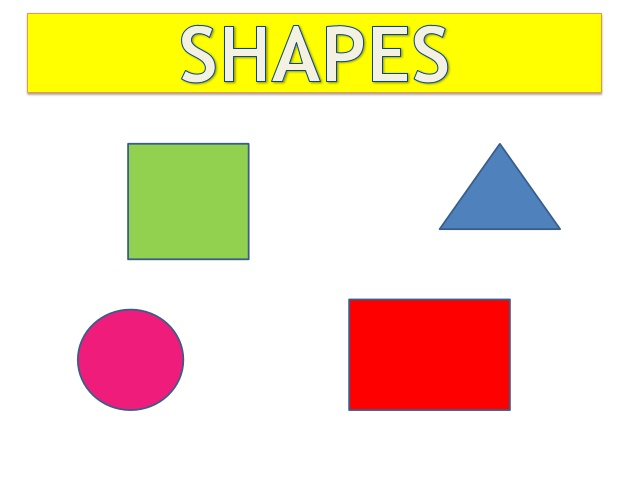
\includegraphics{basic-shapes-english-for-kids-1-638.jpg}}  
\end{figure}

From time to time, you will need some commands. Practically, I use at most 20 commands regularly, and sometimes I need tricky command which I find on the internet. I emphasize again that if you have any question, feel free to ask me.

\end{proof}

\begin{thebibliography}{99} 

\bibitem{wilk} David R. Wilkins: \textit{Getting started with Latex}, \begin{verbatim} http://www.maths.tcd.ie/~dwilkins/LaTeXPrimer/
\end{verbatim}

\bibitem{wiki} \begin{verbatim} http://en.wikibooks.org/wiki/LaTeX \end{verbatim}



\end{thebibliography}



\end{document}
